\chapter{Implementation}
\label{chap:implementation}
This chapter will detail the development and implementation of the automation
platform as well as the configuration of \gls{aci} and vCenter
\section{ACI Configuration}
The initial wizard was used to set up the fabric and bring it up to a level
where configuration can be applied. During the wizard, the first thing to
configure is the fabric membership, where the auto-discovered spines and leafs
are onboarded and registered into \gls{apic}.
One of the most important settings is to configure the spine to perform as a
BGP route reflector, this is because \gls{mp-bgp} is used internally inside of
\gls{aci} to advertise routes. Figure \ref{fig:bgp-reflection} shows how
\gls{as} 65001 was chosen.

\begin{figure}[H]
    
    \centering
    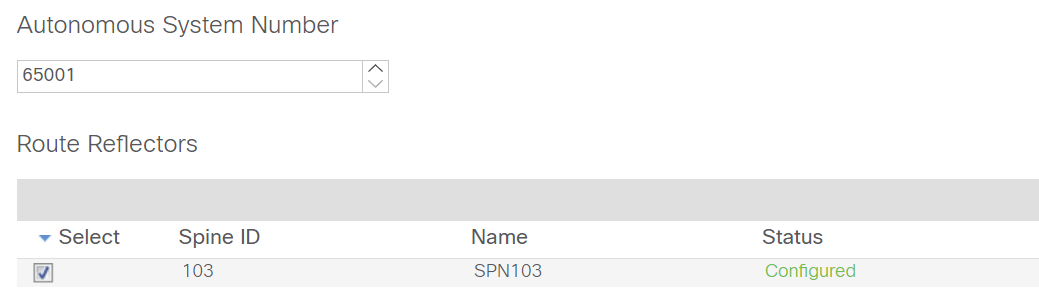
\includegraphics[scale=0.5]{images/bgp-reflection.png}
    
    \caption{BGP Route Relfection}
    \label{fig:bgp-reflection}
\end{figure}

Other settings such as \gls{dns} and \gls{ntp} were configured to ensure that
all devices have name resolution and that all clocks are in sync.
\gls{oob} IP addresses were also configured so that the fabric nodes can be
reached via \gls{ssh} for troubleshooting purposes, figure \ref{fig:aci-oob-ip}
shows the configuration of the \gls{oob} IP addresses.

\begin{figure}[H]
    
    \centering
    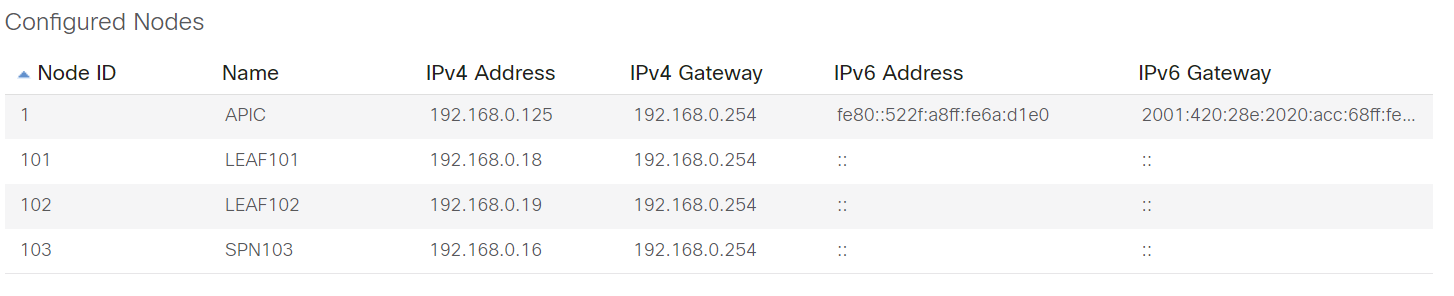
\includegraphics[scale=0.5]{images/aci-oob-ip.png}
    
    \caption{ACI Out of Band IP Configuration}
    \label{fig:aci-oob-ip}
\end{figure}

\subsection{VMware vCenter Integration with ACI}
\gls{aci} provides the handy functionality of being able to integrate with
vCenter and automatically push created \gls{epg}s into vCenter in the form of
\gls{dpg}s with the VLAN tagging being handled automatically.
Firstly, a dynamic VLAN pool was created which is required so that VLANs can
automatically be associated with \gls{epg}s and \gls{dpg}s. Figure
\ref{fig:vmm-integration} shows the configuration of the VMWare integration.

\begin{figure}[H]
    
    \centering
    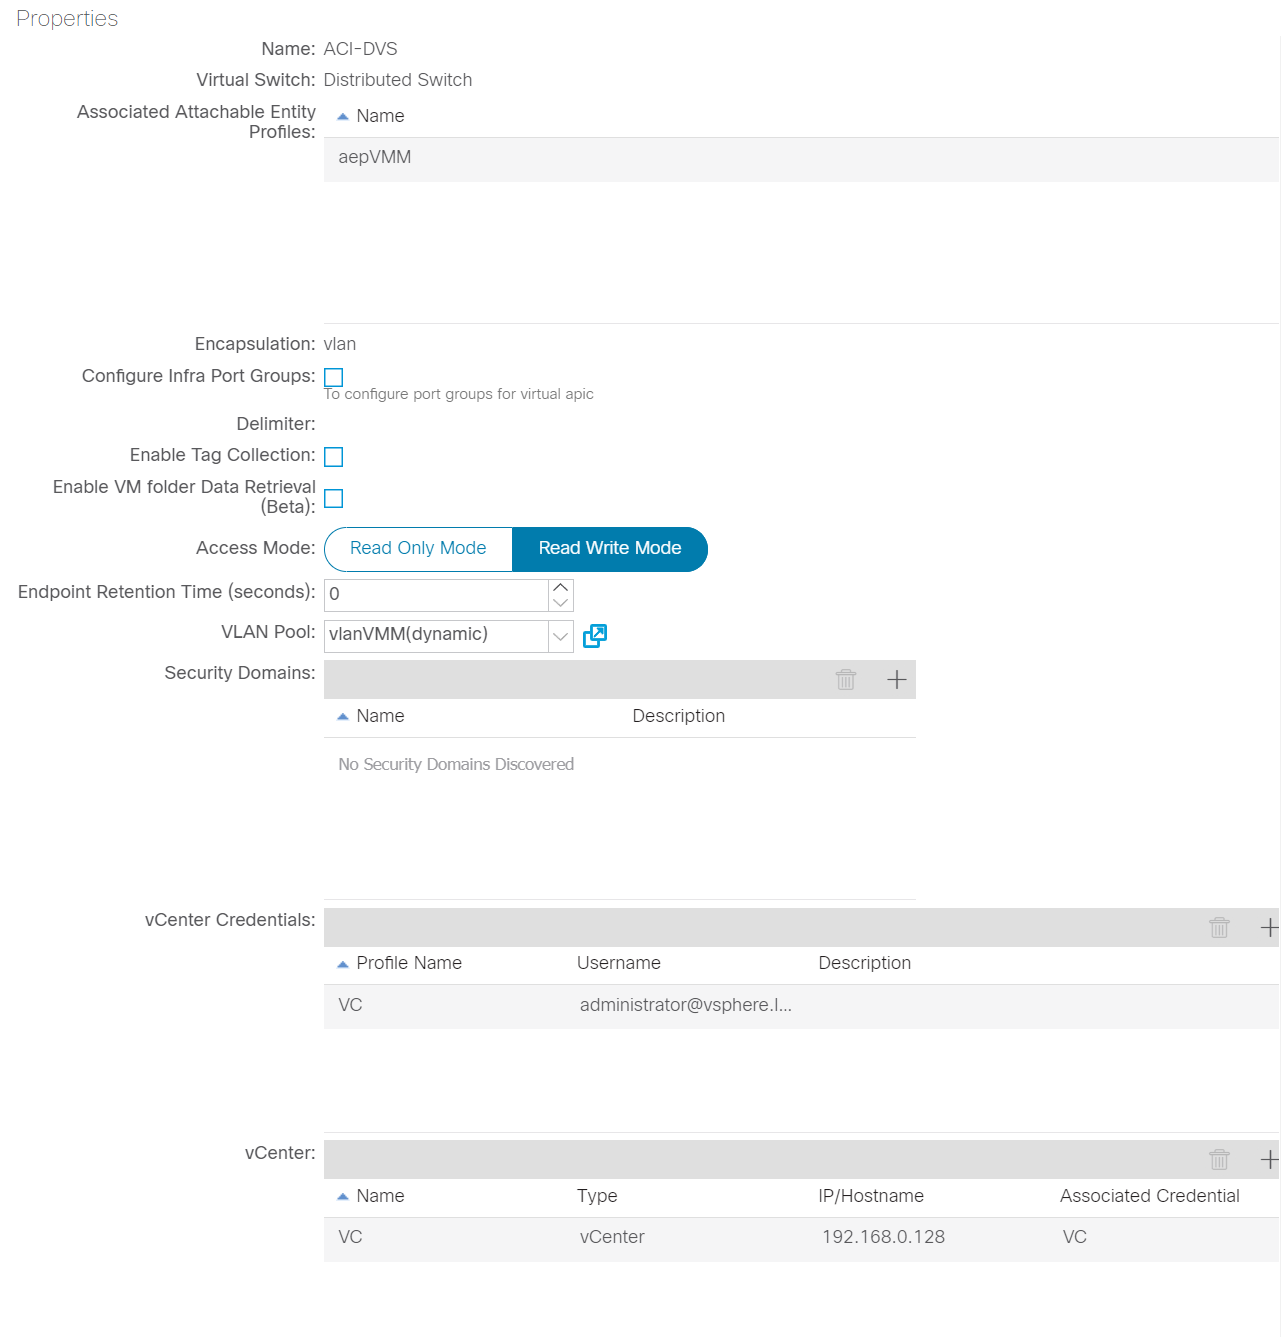
\includegraphics[scale=0.6]{images/vmm-integration.png}
    
    \caption{VMWare Integration Configuration}
    \label{fig:vmm-integration}
\end{figure}

To get the dual-homed connection of the ESXi host to the two leafs operational,
the two leafs must be brought together to form a \gls{vpc} pair.
Firstly, a \gls{vpc} protection group must be created to inform \gls{aci} that
these two leafs should have a keepalive link formed via the spine between them.
\begin{figure}[H]
    
    \centering
    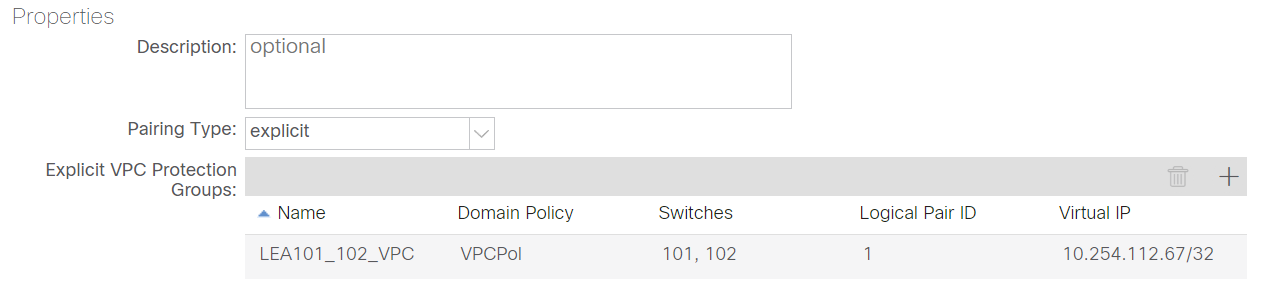
\includegraphics[scale=0.7]{images/vpc-protection.png}
    
    \caption{vPC Protection Group}
    \label{fig:vpc-protection}
\end{figure}

A \gls{vpc} policy group can then be created to associate the VMWare
integration with the \gls{aaep}, and to also configure the interfaces
associated with the group to use LACP.

\begin{figure}[H]
    
    \centering
    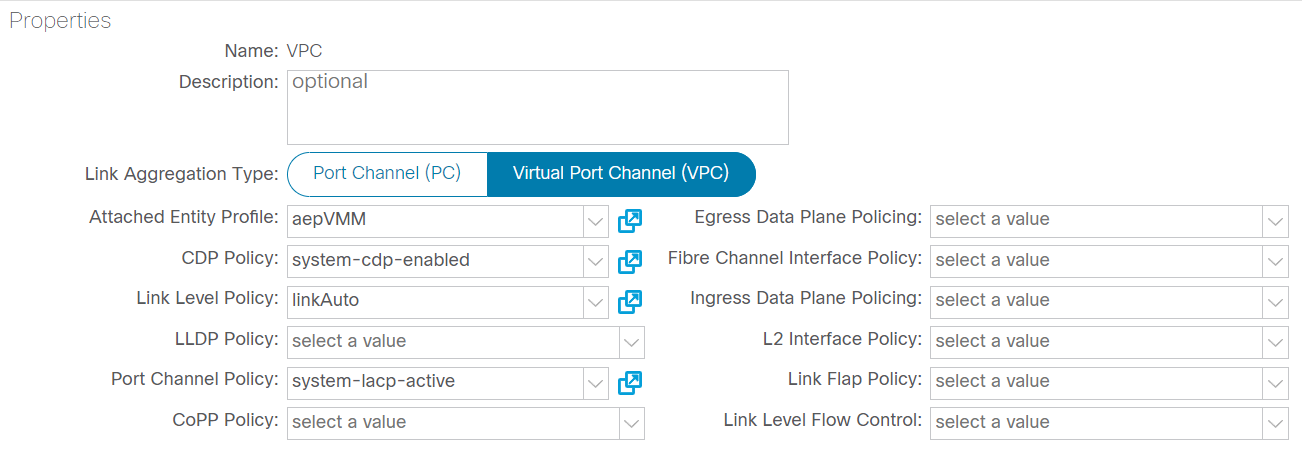
\includegraphics[scale=0.7]{images/vpc-interface-policy.png}
    
    \caption{vPC Interface Policy Group}
    \label{fig:vpc-int-pol}
\end{figure}

This \gls{vpc} policy group can then be applied to the interfaces on the leafs
via an interface profile which is shown in figure
\ref{fig:vpc-interface-assignment}.
\begin{figure}[H]
    
    \centering
    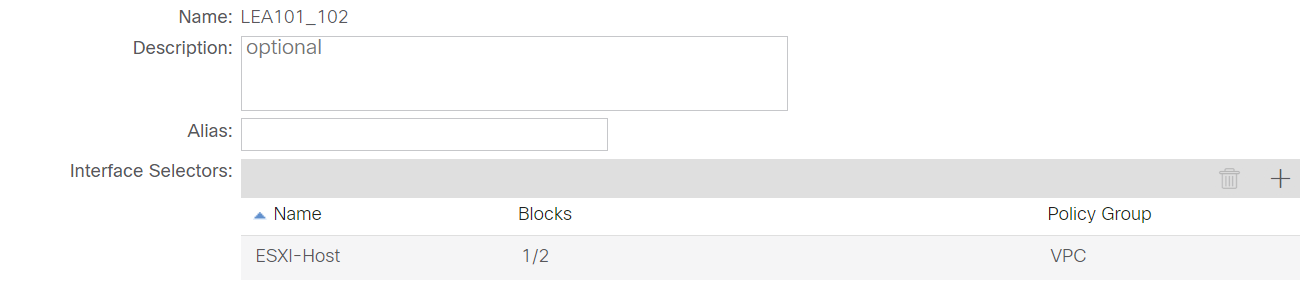
\includegraphics[scale=0.7]{images/vpc-interface-assignment.png}
    
    \caption{vPC Interface Assignment}
    \label{fig:vpc-interface-assignment}
\end{figure}

In vCenter, figure \ref{fig:vcenter-dvs} shows that \gls{aci} has correctly
pushed the \gls{dvs} to vCenter.

\begin{figure}[H]
    
    \centering
    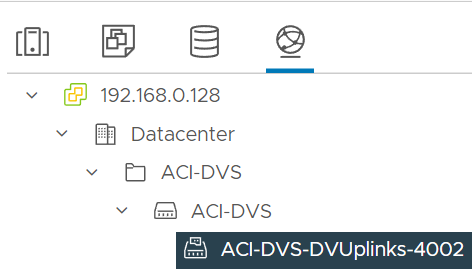
\includegraphics[scale=0.7]{images/vcenter-dvs.png}
    
    \caption{vCenter Distributed Virtual Switch}
    \label{fig:vcenter-dvs}
\end{figure}
Now the uplinks need to be assigned to the \gls{lacp} group that has been
created by ACI. Figure \ref{fig:uplink-lacp} shows the configuration of the
uplinks to use LACP.

\begin{figure}[H]
    
    \centering
    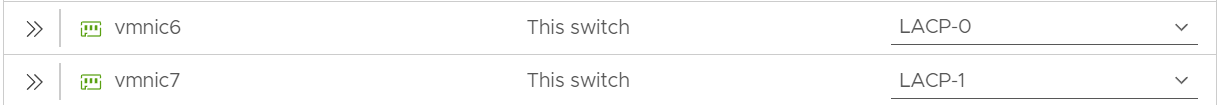
\includegraphics[scale=0.7]{images/lacp-interface-assignment.png}
    
    \caption{Uplink LACP Configuration}
    \label{fig:uplink-lacp}
\end{figure}
The command \verb|fab 101 show vpc extended| can then be executed on the \gls{apic} via \gls{ssh} to retrieve the status of all \gls{vpc} present on leaf 101.
\begin{figure}[H]
    \begin{small}
        \begin{verbatim}
    vPC status
-----------------------------------------------------------------------------
id   Port   Status Consistency Reason      Active vlans         Bndl Grp Name
--   ----   ------ ----------- ------      -------------------- -------------
343  Po3    up     success     success     1135,1168-1169,1200- VPC
                                            1201

    \end{verbatim}
    \end{small}
    \caption{vPC Status on Leaf 101}
    \label{fig:vpc-status}
\end{figure}


\subsection{TEN\textunderscore INFRA Tenant Setup}
With vCenter integration complete, the tenant can now be created that will house all policies related to the infrastructure of the testbed. All of the \gls{vrf}s/\gls{bd}s/\gls{epg}s were created in accordance with the topology shown in figure \ref{fig:epg-topology}.

To get external connectivity working with the \gls{nat} router that will be provisioned inside vCenter, L3Out configuration must be created. Figure \ref{fig:l3out} shows the configuration of the L3Out that will be used for the Infra \gls{vrf}, an \gls{ospf} area of 1 has been specified. A floating \gls{svi} has been utilised so that the VMWare integration configured earlier can be used to pass the L3out \gls{epg} to vCenter automatically. A new static VLAN pool was created along with a new L3 domain. This L3 domain was then added to the VMWare integration so that L3Outs can then use the VMWare virtual domain.

\begin{figure}[H]
    
    \centering
    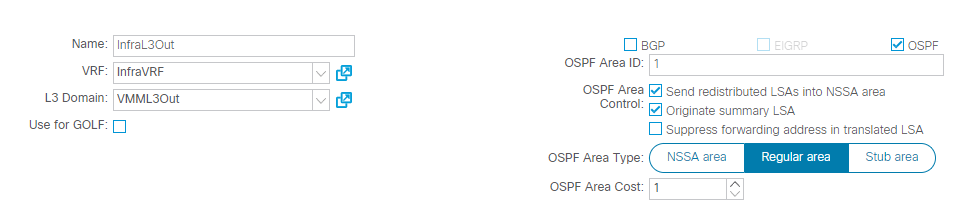
\includegraphics[scale=0.6]{images/InfraL3Out.png}
    
    \caption{Infra L3Out Configuration}
    \label{fig:l3out}
\end{figure}

\begin{figure}[H]
    
    \centering
    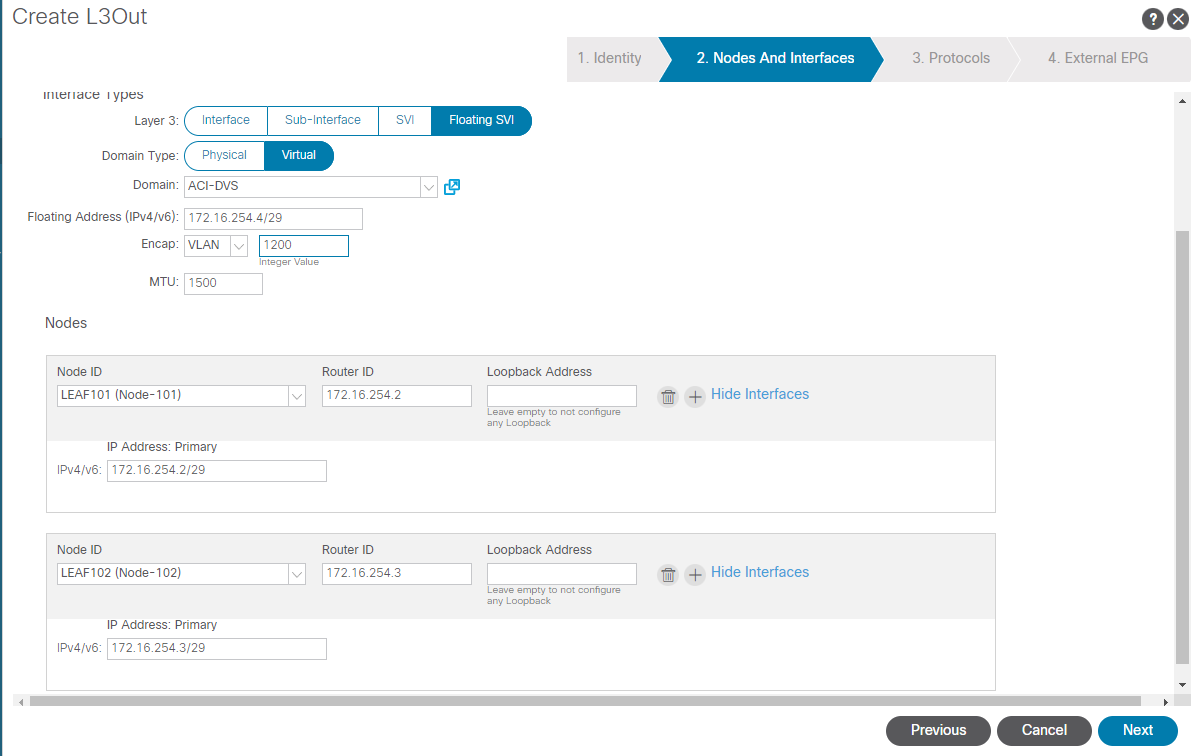
\includegraphics[scale=0.47]{images/InfraL3OutNodes.png}
    
    \caption{Adding the leafs to the L3Out}
    \label{fig:l3out-nodes}
\end{figure}

It is then important to assign the L3out interface profiles to the enhanced \gls{lacp} group so that the OSPF and traffic flow utilise \gls{lacp} to vCenter correctly. Figure \ref{fig:l3out-lacp} shows the configuration of the L3Out interface profiles.

\begin{figure}[H]
    
    \centering
    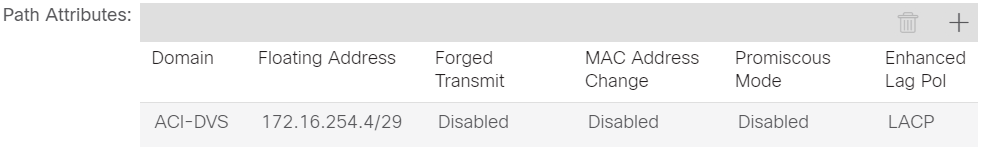
\includegraphics[scale=0.8]{images/l3out-lacp.png}
    
    \caption{L3Out Interface Profile Configuration}
    \label{fig:l3out-lacp}
\end{figure}

The same process will be repeated for the InternetL3Out for the InternetVRF.

The \gls{nat} router can then be deployed and attached to the L3Out \gls{epg}s via the \gls{dpg}s that have been pushed to vCenter by \gls{aci}.

\subsubsection{NAT Router Configuration}

For virtual routing, the Cisco CSR1000v Virtual Router was chosen. The interfaces were configured with IP addresses that are present in the subnets that were used in the earlier L3Out configuration. \gls{ospf} was also configured so that the routes to and from \gls{aci} are advertised correctly. The following \gls{ospf} configuration was used for the \gls{nat} router.

\begin{figure}[H]
    \begin{verbatim}
        router ospf 1
        passive-interface default
        no passive-interface GigabitEthernet1
        network 172.16.254.0 0.0.0.7 area 1
        default-information originate
        !
        router ospf 2
        passive-interface default
        no passive-interface GigabitEthernet2
        network 172.16.254.8 0.0.0.7 area 2
        default-information originate
    \end{verbatim}
    \caption{NAT Router OSPF Configuration}
    \label{fig:nat-ospf}
\end{figure}

To verify the \gls{ospf} configuration is working correctly, the following command and output was executed on the \gls{nat} router.

\begin{figure}[H]
    \centering
    \begin{small}
        \begin{verbatim}
InternetRouter#show ip ospf neighbor

Neighbor ID    Pri  State      Dead Time   Address         Interface
172.16.254.10    1  FULL/BDR   00:00:35    172.16.254.10   GigabitEthernet2
172.16.254.11    1  FULL/DR    00:00:33    172.16.254.11   GigabitEthernet2
172.16.254.2     1  FULL/BDR   00:00:39    172.16.254.2    GigabitEthernet1
172.16.254.3     1  FULL/DR    00:00:32    172.16.254.3    GigabitEthernet1

    \end{verbatim}
    \end{small}
    \caption{NAT Router OSPF Neighbors}
    \label{fig:nat-ospf-db}
\end{figure}

Basic \gls{nat} overload can then be configured for all subnets present on \gls{aci} so that the various bridge domains now have internet via the router.

\section{vCenter Configuration}
As \gls{aci} has configured the virtual switch and port groups for us, the only configuration required is to make a \gls{vm} that will serve as a project router template that the automation scripts will then clone. Due to a limitation with the vCenter \gls{rest} \gls{api}, the \gls{vm} to be cloned will be a regular \gls{vm} and not a template. This is because the \gls{rest} \gls{api} does not support cloning templates.

The router will have 3 ethernet interfaces:
\begin{itemize}
    \item GigabitEthernet 0 - Project Network
          \begin{itemize}
              \item IP Address set by automation platform.
          \end{itemize}
    \item GigabitEthernet 1 - WAN Uplink
          \begin{itemize}
              \item IP Address set by automation platform.
          \end{itemize}
    \item GigabitEthernet 2 - Management
          \begin{itemize}
              \item IP Address obtained by DHCP so the automation platform can connect.
          \end{itemize}
\end{itemize}


The router will need to obtain an IP address from \gls{dhcp} on the CSRMgmt \gls{epg} so that the automation platform can connect via RESTCONF. The router will also have an interface in the Internet \gls{epg} and then the other interface will be set to the quarantine \gls{dpg} so that it can be assigned to the \gls{epg} created for the project by the automation platform. \gls{nat} overload can also be preconfigured on the router so that the project can access the internet, however, the \gls{nat} \gls{acl} will need to be configured via RESTCONF by the automation platform.

\section{Automation Platform}
Both backend and frontend features were developed simultaneously as that was the most efficient way of development. Instead of backend and frontend implementation detailed separately, development of features will instead be covered.
\subsection{Packages}
To accelerate development, many packages and libraries were used.
\subsubsection{Next.js}
Next.js is based on React and is a framework for server-side rendering and static site generation. It is used to create the frontend of the automation platform. It features many benefits over using plain React, such as the ability to pre-render many parts of the web application resulting in a reduction of load times upon page load. TypeScript is also supported which was used to aid development by enforcing the usage of types when defining variables and functions.

\subsubsection{Tailwind CSS}
Tailwind CSS is a utility-first CSS framework. It is used to style the frontend of the automation platform. It has many benefits over plain CSS, such as the ability to rapidly create a responsive UI through the use of pre-defined classes. The Flowbite React package was also utilised, which is a library of components that utilise Tailwind CSS for styling. Tailwind also features dark mode support which was used to create a dark theme for the automation platform.

\subsubsection{React Flow}
React Flow is a library that provides the ability to create and programmatically define flowcharts within React. It is used to create the rackspace layout feature and is the core of the automation platform. By using React Flow, development time was greatly reduced. It also has features such as the ability to define custom nodes to be displayed, which is required to get the desired look, feel and functionality for the application.

\subsubsection{Laravel}
Laravel is a PHP framework that makes it quick and easy to create feature-rich \gls{api}s which is why it was chosen. It features an easy-to-use routing system for easily routing \gls{api} requests to the correct controller classes. It also makes use of the Eloquent \gls{orm} which makes it easy to create and query the database. The inbuilt Guzzle \gls{http} client also makes interacting with the various \gls{api}s required to build the automation scripts easy and simple.

\subsection{Recreation of Rackspace}
To allow for the recreation of the rackspace in a map-like user interface, React Flow was used with custom nodes that represent racks. To save the positions of the racks in 2D space, the following \gls{api} endpoints were created:
\begin{table}[htbp]
    \centering
    \begin{tabular}{@{} c c c @{}}
        \toprule
        \textbf{API Path}     & \textbf{Method} & \textbf{Description} \\
        \midrule
        \texttt{/node/\{id\}} & \texttt{GET}    & Get a node by ID     \\
        \texttt{/node/\{id\}} & \texttt{PATCH}  & Update a node by ID  \\
        \texttt{/node/\{id\}} & \texttt{DELETE} & Delete a node by ID  \\
        \texttt{/node}        & \texttt{GET}    & Get all nodes        \\
        \texttt{/node}        & \texttt{POST}   & Create a new node    \\
        \bottomrule
    \end{tabular}
    \caption{API Routing Table}
\end{table}
As React Flow uses the term 'node' to refer to the individual elements in the flowchart, the \gls{api} endpoints were also named 'node' to avoid confusion. Every time a node is moved on the flowchart, the \gls{api} is called to update the position of the node in the database. 

The ability to add labels to the rackspace representation was also deemed an important feature, as it would allow for useful pieces of information to be placed on the map. To facilitate this, a new custom node was created that just displays text. Shown below in figure \ref{fig:rackspace-layout} is the rackspace layout feature with a label used to illustrate the name of the row.

\begin{figure}[H]
    \centering
    \includegraphics[scale=0.7]{rackspace-layout.png}
    \caption{Rackspace Layout}
    \label{fig:rackspace-layout}
\end{figure}

React Flow provides a handy interface for allowing custom nodes to be dragged and dropped, allowing for a user-friendly way to add racks and labels to the space. Shown in figure \ref{fig:drag-drop} is the utility panel where racks and labels can be dragged and dropped onto the rackspace representation.

\begin{figure}[H]
    \centering
    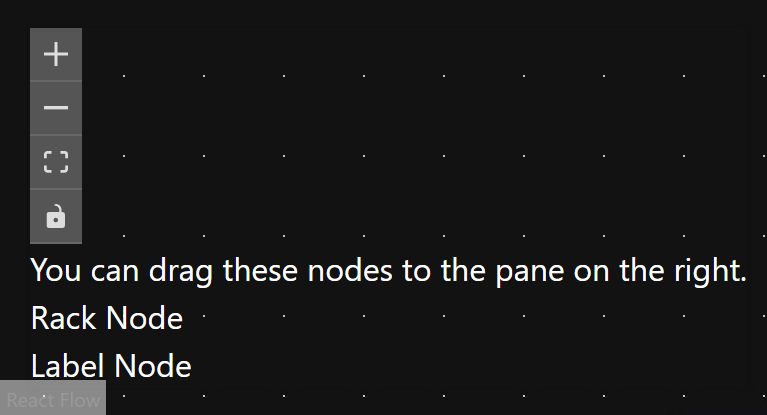
\includegraphics[scale=0.7]{drag-drop.png}
    \caption{Drag and Drop}
    \label{fig:drag-drop}
\end{figure}

\subsection{Initial ACI Integration}
\subsubsection{Fabric Nodes}
With the ability to add racks to the space, the next feature to be developed was the integration with \gls{aci}. As the premise of the application is that each rack has a top of rack switch, the automation platform needs to be able to pull all of the available leafs and \gls{fex}s from the \gls{aci} fabric so that they can then be assigned to a rack. Because \gls{aci} treats a \gls{fex} as an extension of a leaf node, some logic is required to differentiate between the two.
To retrieve \gls{fex}s, a list of all leaf nodes can be retrieved from \gls{aci}, the list of leaf nodes can then be iterated over and the following \gls{api} endpoint can be used to retrieve a list of all \gls{fex}s attached to the leaf node:
\begin{verbatim}
https://apic-ip/api/node/class/topology/pod-1/node-{leafID}/eqptExtCh.json
\end{verbatim}

The returned objects are \gls{fex}s that are attached to the leaf with the given ID. This information can be stored in the database with the \verb|role| column used to differentiate between a leaf and \gls{fex}. The column \verb|aci_parent_id| is also set to the parent leaf as that will be required for subsequent \gls{api} calls.

With the nodes synced to the database, the next step is to provide the user to specify which interface profiles should be used by the automation platform to select the access ports on the leafs and \gls{fex}s. A requirement of the platform will be that an interface profile that belongs to a single node will have to be manually created as it is not easy to automate the creation of this. Two \gls{api} queries will have to be made as \gls{fex} and leaf interface profiles are treated separately. The following \gls{api} endpoints were used to retrieve this information:
\begin{verbatim}
https://apic-ip/api/node/mo/uni/infra.json?query-
target=subtree&target-subtree-class=infraAccPortP

https://apic-ip/api/node/mo/uni/infra.json?query-
target=subtree&target-subtree-class=infraFexP
\end{verbatim}

A basic modal can then be created with a dynamic form that will allow the user to map the fabric nodes to an interface profile. Figure \ref{fig:interfaceprof-mapping} shows the modal with the interface profile mapping form.

\begin{figure}[H]
    \centering
    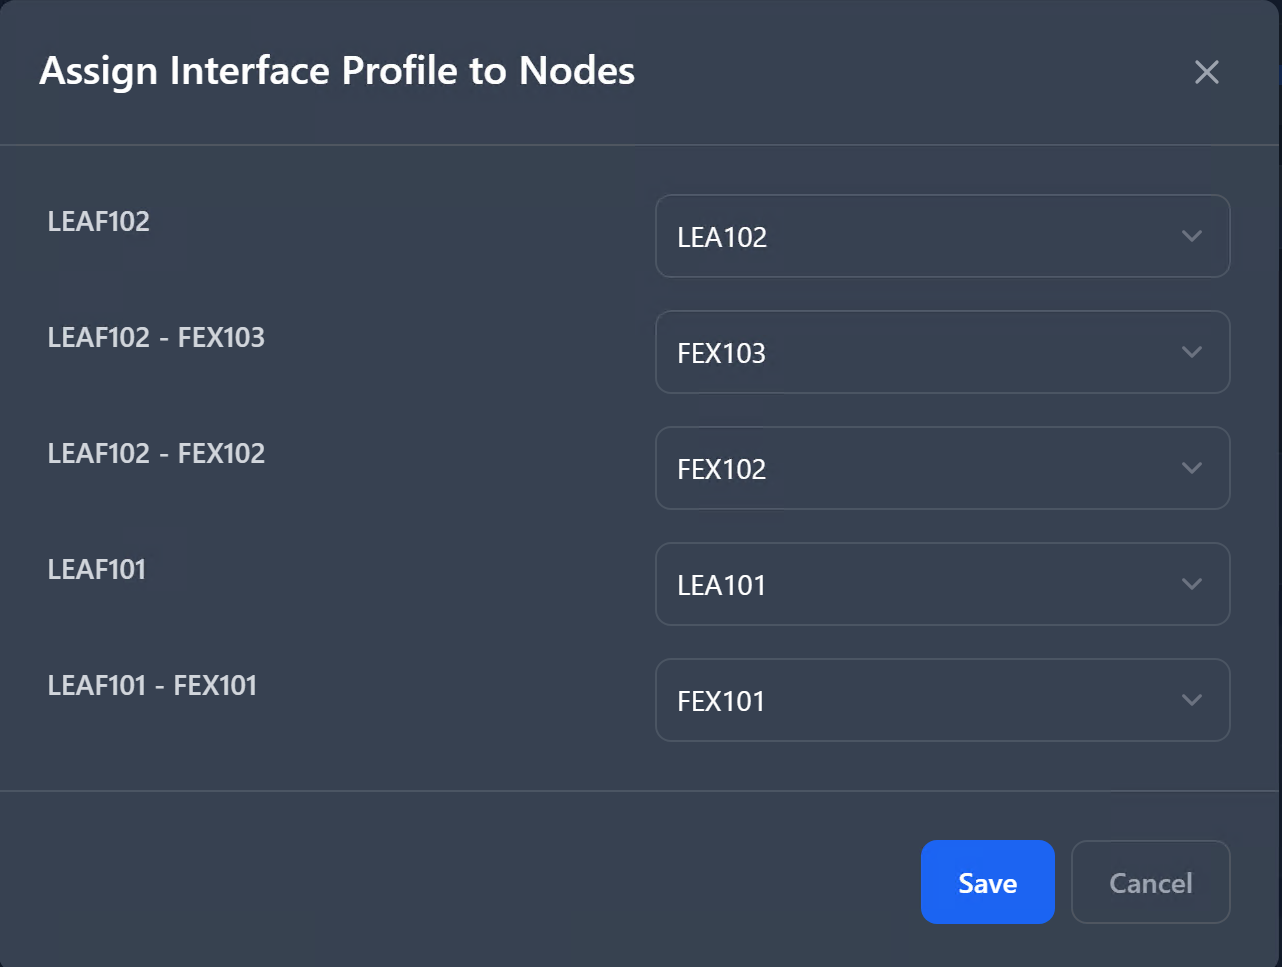
\includegraphics[scale=0.7]{interfaceprof-mapping.png}
    \caption{Interface Profile Mapping}
    \label{fig:interfaceprof-mapping}
\end{figure}

The distinguished name of the interface profile selected can then be stored in the corresponding \verb|int_profile| column of the fabric node.

\subsubsection{VLAN Pools}
So that the automation platform can assign unique VLANs to projects, the correct VLAN pool from \gls{aci} must be used so that the physical domain that the automation platform will create is attached to the correct VLAN pool. The list of valid VLAN pools will then be presented to the user in the form of a dropdown menu where the desired VLAN pool can be set. Figure \ref{fig:vlan-pool-selection} shows the selection dropdown.

\begin{figure}[H]
    \centering
    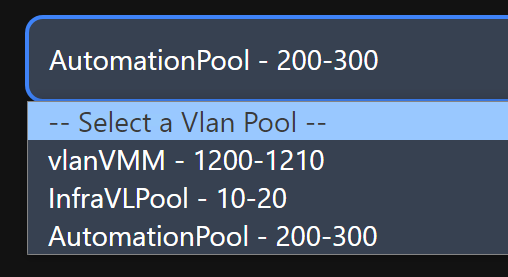
\includegraphics[scale=0.7]{vlan-pool-selection.png}
    \caption{VLAN Pool Selection}
    \label{fig:vlan-pool-selection}
\end{figure}

The selected VLAN pool can then be saved in the database using the \verb|project_pool| column set to \verb|true| for the corresponding pool. The future project logic will then be able to retrieve the start and ending VLAN that can be used and allocate individual VLANs to projects.

\subsection{Terminal Servers}
Terminal servers will have a dedicated management page so that the status of connected terminal servers can be monitored. Cisco IOS-XE has an inbuilt RESTCONF server which will be used to retrieve and push configuration to the devices. A form modal to consume data was created which is shown in figure \ref{fig:terminal-server-form}.

\begin{figure}[H]
    \centering
    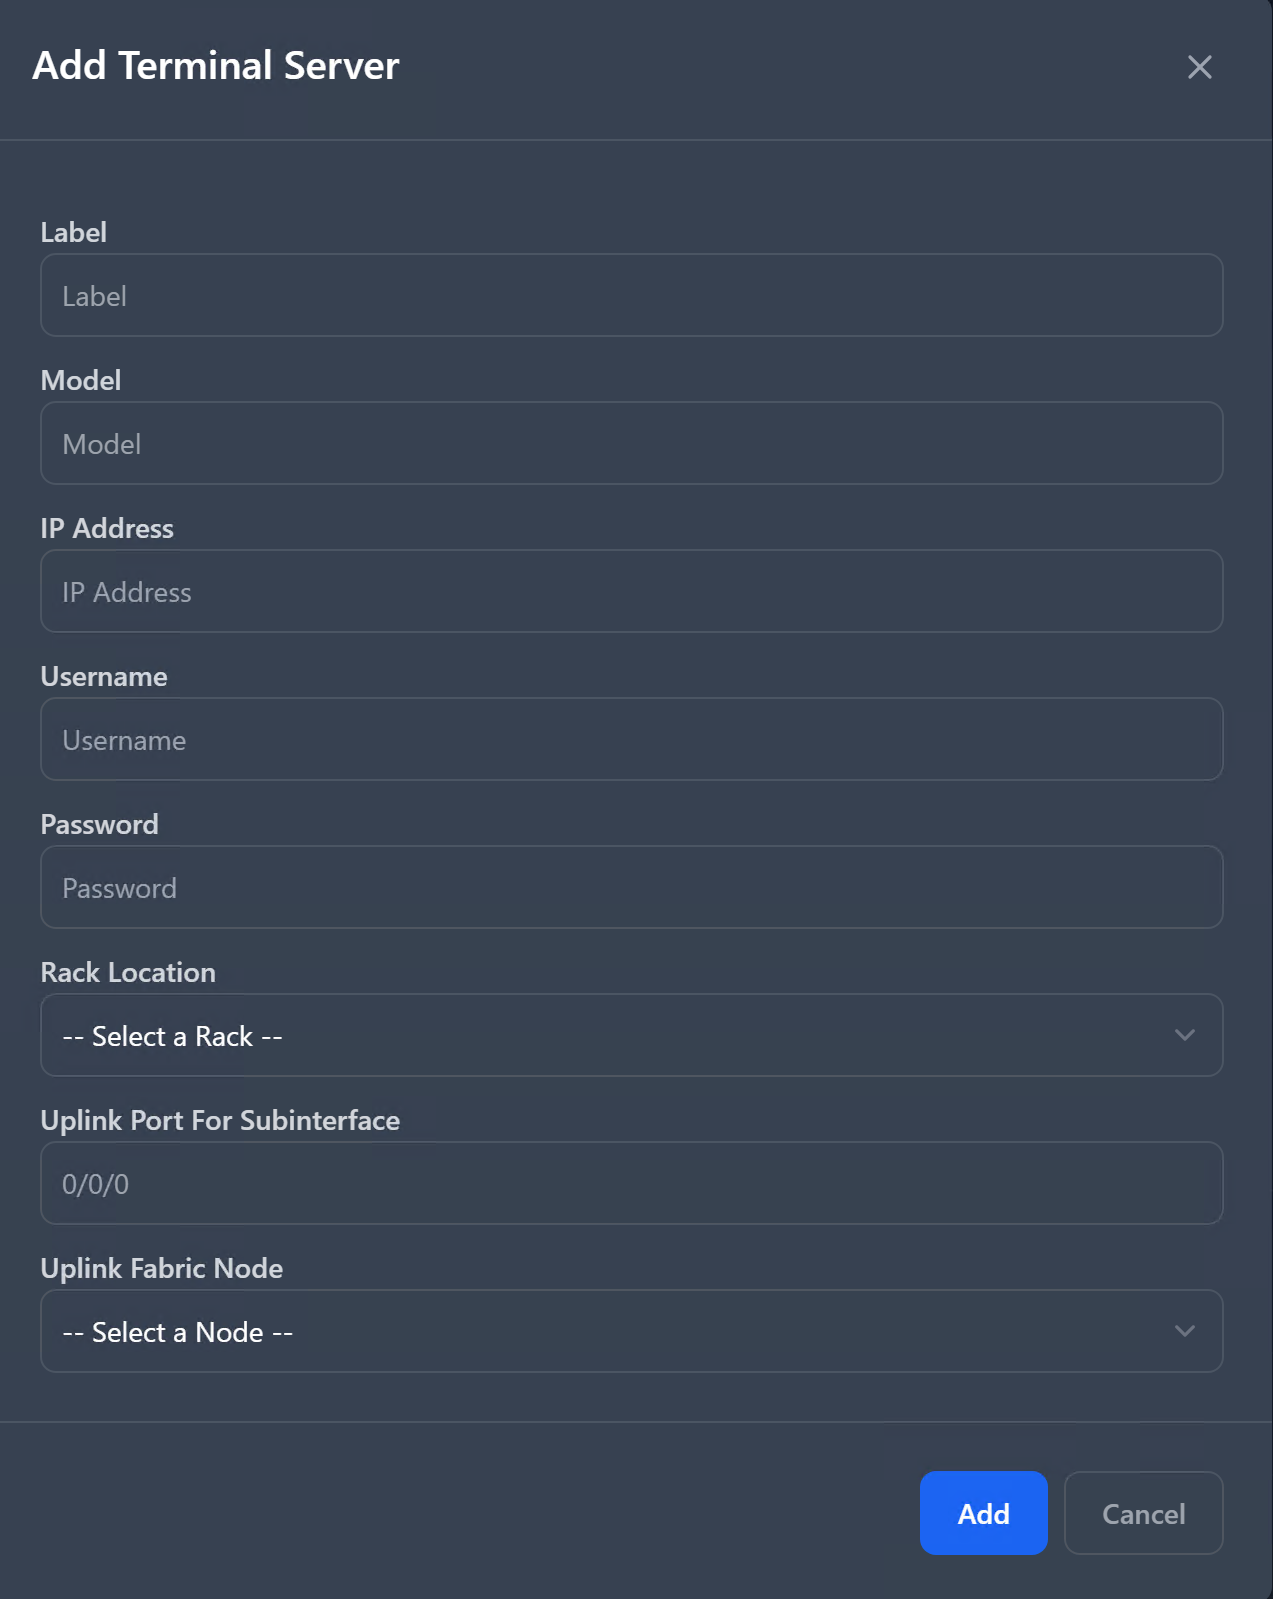
\includegraphics[scale=0.5]{add-ts.png}
    \caption{Terminal Server Addition Form}
    \label{fig:terminal-server-form}
\end{figure}

The notable features are the ability to assign the newly created terminal server straight to a rack, although that feature will also be added to the rackspace view.
The port that is connected to the fabric from the terminal server will need to be manually provided, as the automation scripts will need to create sub-interfaces on top of that interface to facilitate communication to the project network.
The port on the side of that link, the fabric side, will also need to be specified so that the automation scripts can create a trunk interface. The username and password to gain access to the terminal server are also required to be entered by the user.

\subsection{Rack ACI Integration}
As the premise of the automation platform is the ability to automatically include racks into a project's network, the platform needs to be aware of which fabric nodes belong to which rack. To achieve this easily, it was determined that the best method would be to provide an 'edit rack' modal that can be accessed by hovering over a rack. Figure \ref{fig:edit-rack-popover} shows the popover that appears when hovering over a rack.

\begin{figure}[H]
    \centering
    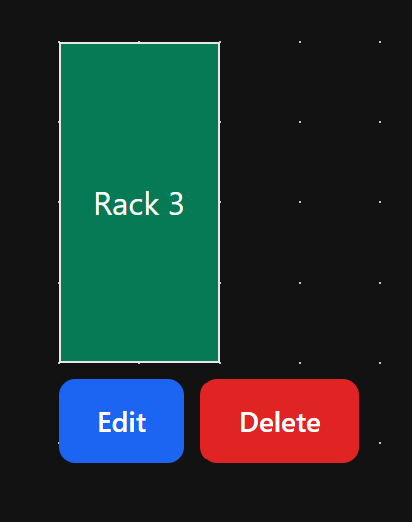
\includegraphics[scale=0.7]{edit-rack-popover.png}
    \caption{Edit Rack Popover}
    \label{fig:edit-rack-popover}
\end{figure}

The ability to change a rack's name, as well as associate a fabric node and terminal server was provided in the edit modal, which is shown in figure \ref{fig:edit-rack-modal}.

\begin{figure}[H]
    \centering
    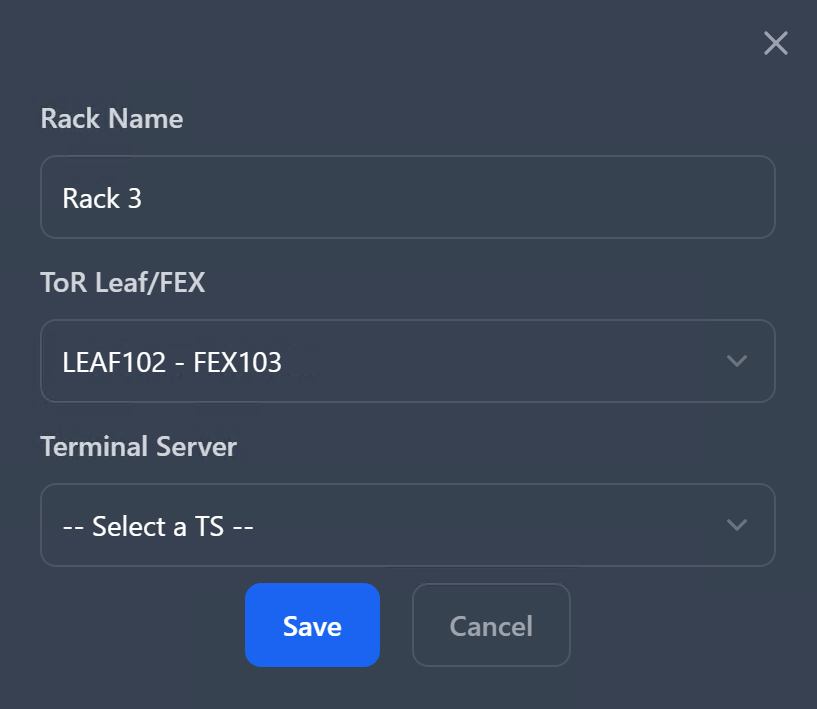
\includegraphics[scale=0.6]{edit-rack-modal.png}
    \caption{Edit Rack Modal}
    \label{fig:edit-rack-modal}
\end{figure}

The logic to only allow a single fabric node and terminal server to a single rack was also incorporated to prevent user error. The \verb|rack_id| column of the fabric node and terminal server tables were updated to reflect the rack that they were assigned to.

\subsection{Project Creation}
The final user-facing feature to be developed is the ability to create projects, which is the main feature of the automation platform. The user will have the ability to create and edit projects as well as delete them. The edit functionality will include adding and removing racks from the project, to facilitate project expansion and contraction which is a very common requirement.

A modal was decided upon as being the most user-friendly way of adding and editing projects. A multi-stage form that guides the user through the process of onboarding the project was also decided upon. The flow will be as follows:
\begin{enumerate}
    \item The user will be presented with a form to enter the project name and description.
    \item The user will be presented with a list of racks that are available to be added to the project.
    \item The user will be asked to specify a subnet to be used in the project network along with a WAN IP address. If no project subnet is specified, the next available subnet will be automatically assigned.
\end{enumerate}
Shown in figure \ref{fig:add-project-racks} is the modal form section that allows the user to select the racks that the project will occupy.

\begin{figure}[H]
    \centering
    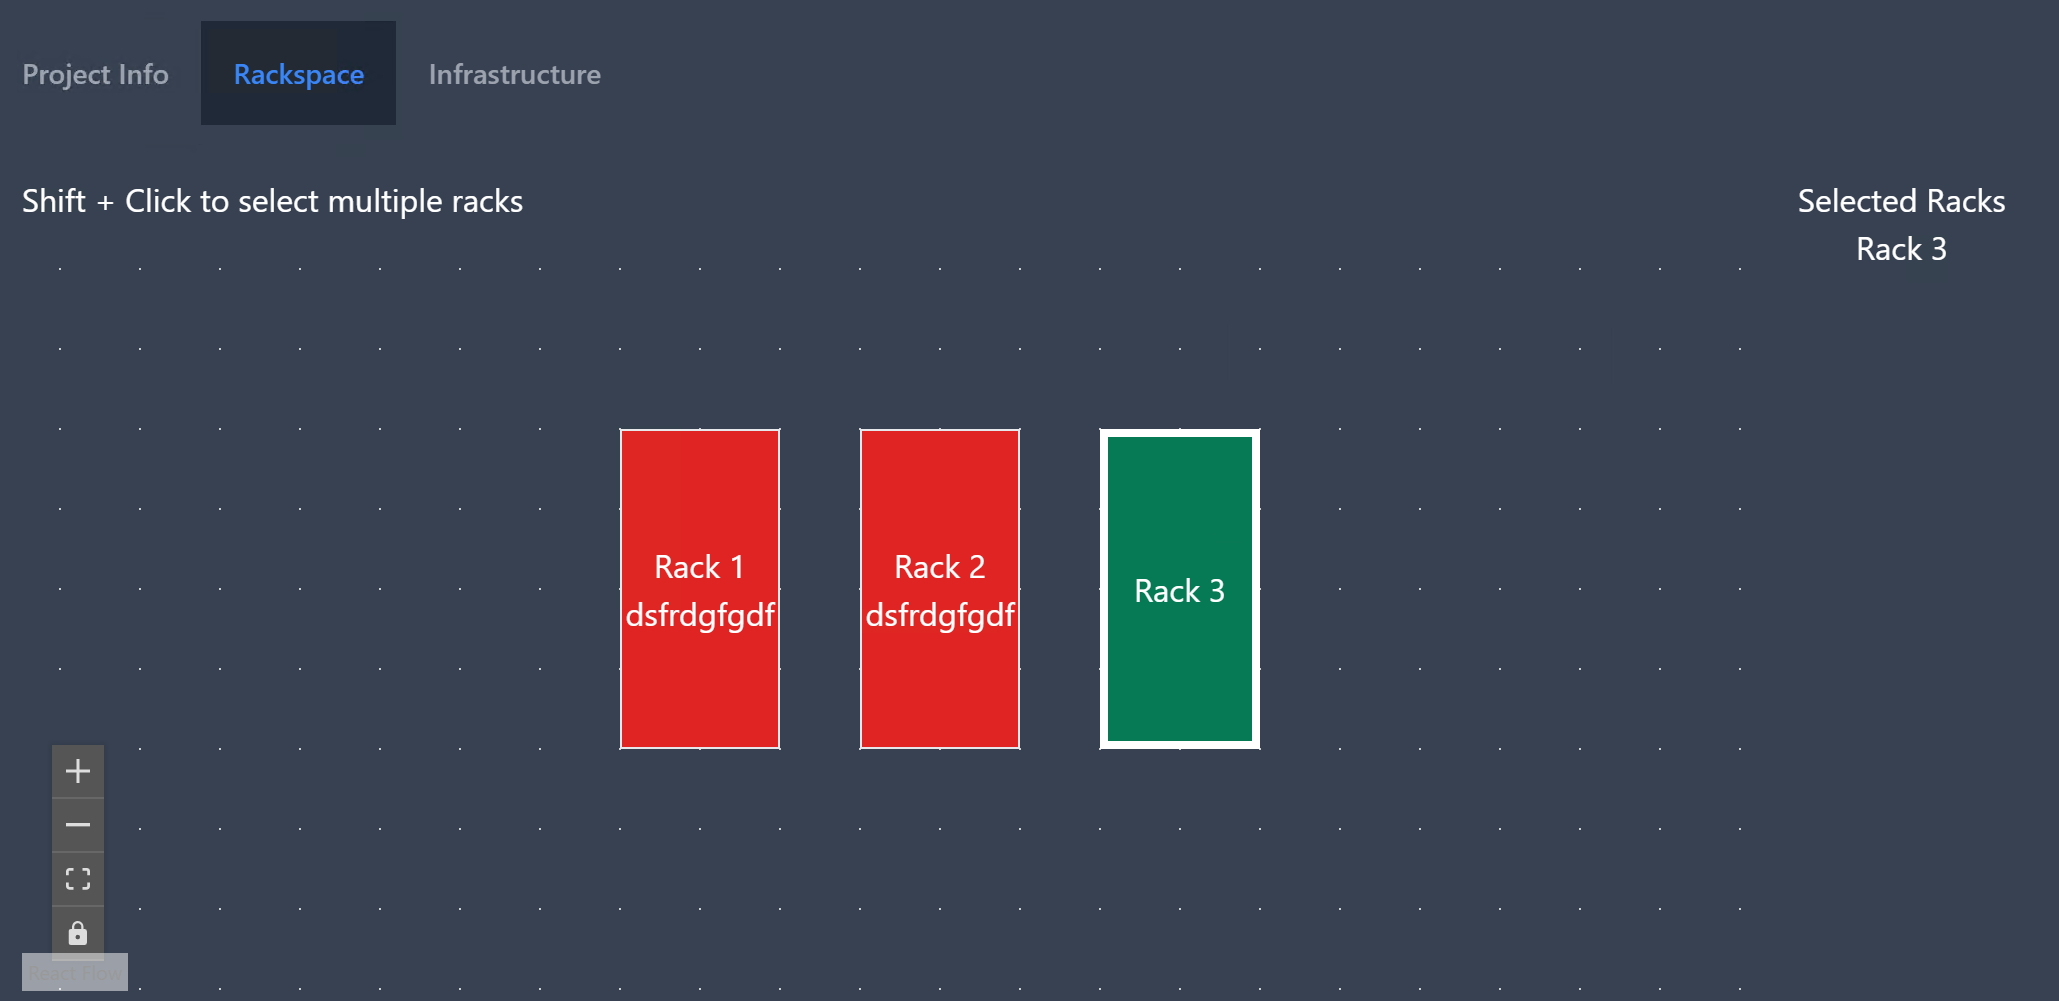
\includegraphics[scale=0.4]{add-project-racks.png}
    \caption{Add Project Racks}
    \label{fig:add-project-racks}
\end{figure}

Because of the componentised nature of React, the rackspace layout can just be imported again instead of redefining all code and properties. The racks shown in red are occupied by another project, and thus cannot be included in a newly created project. The form for specifying IP addressing is shown below.

\begin{figure}[H]
    \centering
    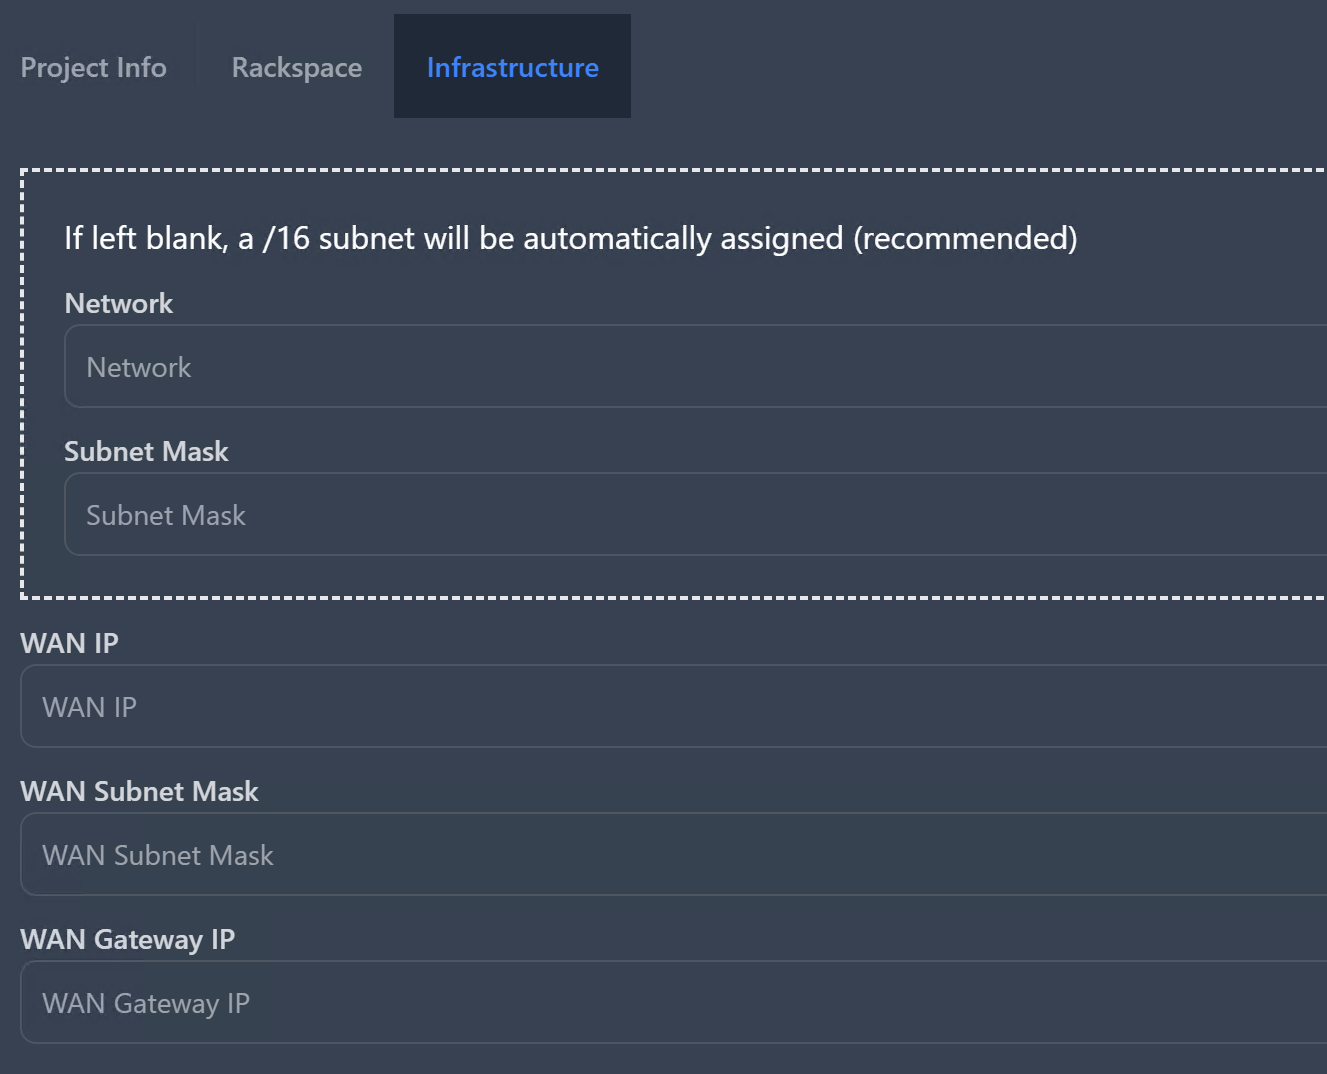
\includegraphics[scale=0.6]{add-project-infrastructure.png}
    \caption{Specifying project IP addressing}
    \label{fig:add-project-infrastructure}
\end{figure}

The same modal layout is used for editing a project, however, the logic is revised to allow racks to be deselected and removed from the project, at the same time as allowing new racks to be added.

\subsection{Project Automation}
With the ability to create projects, the automation platform needs to be able to automatically create the project's network infrastructure. To perform this, Laravel Queues were decided upon, as they allow tasks and \gls{api} queries to be performed outside of the process that responds to the user's request. This allows the user to continue using the platform while the automation scripts are running in the background.

The first step when provisioning a project is to configure the \gls{aci} fabric, as that will be required before any \gls{vm}s can be created and attached to the project network.

\begin{figure}[H]
    \begin{lstlisting}[basicstyle=\scriptsize]
{
    $aciClient = new ACIClient();
    $vmWare = new vSphereClient();
    $project = Project::find($this->projectId);
    if ($aciClient->createTenant($this->projectName)) {
        if ($aciClient->createBD($this->projectName)) {
            if ($aciClient->createAP($this->projectName)) {
                if ($aciClient->createEPG($this->projectName)) {
                    if ($aciClient->associatePhysDom($this->projectName)) {
                        if ($aciClient->deployToNodes($this->projectId)) {
                            $project->status = 'VMware';
                            $project->save();
                            if ($vmWare->deployProjectRouter($this->projectName,
                            $this->projectId)) {
                                VirtualRouterProvision::dispatch($this->projectId)
                                ->delay(Carbon::now()->addSeconds(140));

                                TSProvision::dispatch($this->projectId);
                                return true;
                            }
                        }
                    }
                }
            }
        }
    }
    $project->status = 'Error';
    $project->save();
    return false;
}
\end{lstlisting}
    \caption{Project Creation Job}
    \label{fig:project-creation-job}
\end{figure}

Figure \ref{fig:project-creation-job} shows the job that is dispatched when a project is created. The job performs the following actions:
\begin{enumerate}
    \item Creates the tenant in \gls{aci} where all network configurations related to the project will be stored. The project \gls{vrf} will automatically be created with this \gls{api} call.
    \item Creates the bridge domain to allow L2 communication between attached ports and \gls{vm}s.
    \item Creates the application profile that will house the \gls{epg}.
    \item Creates the \gls{epg} that will be used to attach static ports and \gls{vm}s to the project network.
    \item Associates the created \gls{epg} with the Automation and Terminal Server physical domains. It also associates with the VMware integration domain so that the created \gls{epg} is automatically extended into VMware vCenter.
    \item The fabric node and their ports that are attached to the member racks that the project has been allocated to are then added into the \gls{epg}s static mapping.
    \item The project router is then deployed through the use of vCenters ability to clone a \gls{vm} using the \gls{api}. When the \gls{vm} has been cloned, a new job is dispatched with an initial delay of 140 seconds. This job will find the newly created \gls{vm}s IP address via VMWare guest tools and then configure the \gls{vm} with the appropriate network configuration. The delay is added to give the \gls{vm} time to boot up and acquire an IP from \gls{dhcp}. 
\end{enumerate}
Shown in figure \ref{fig:project-router-configuration-job} is the job that is dispatched from the create project job.
\begin{figure}[H]
    \begin{lstlisting}[basicstyle=\scriptsize]
        {
        $vmWare = new vSphereClient();
        $project = Project::with('projectRouter')->find($this->projectId);
        for ($i = 0; $i < 10; $i++) {
            $routerIp = $vmWare->getVmIp($project->projectRouter->vm_id);
            if ($routerIp !== false && $routerIp != '0.0.0.0') {
                $httpClient = new IOSXEClient($routerIp);
                if ($httpClient->connectionTest()) {
                    if ($httpClient->setHostname($project->name . '-CSR') &&
                        $httpClient->setAddresses($project->projectRouter->ip,
                        $project->projectRouter->subnet_mask, $project->network,
                        $project->subnet_mask, $project->projectRouter->gateway)) {

                        $httpClient->save();
                        $project->status = 'Provisioned';
                        $project->save();
                        return true;
                    } else {
                        $project->status = 'Error';
                        $project->save();
                        return false;
                    }
                } else {
                    sleep(10);
                }
            } else {
                sleep(10);
            }
        }
        return false;
        }
    \end{lstlisting}
    \caption{Project Router Configuration Job}
    \label{fig:project-router-configuration-job}
\end{figure}

The first step the algorithm takes is to enter a for loop that will iterate for a maximum of 10 times. The vCenter \gls{api} will be contacted to retrieve a list of IP addresses belonging to a specific \gls{vm}. As the ID of each project router associated with a project is stored in the database, this ID can be used to get the IP address of a project's router. If the \gls{vm} has not yet received an IP address, then the loop will sleep for 10 seconds and then try again. Once an IP address has been received and registered by vCenter, the next step can be performed. The IP address is then used to create a new instance of the IOS-XE client, which is used to configure the router via RESTCONF. The hostname and addresses are pulled from the database and pushed to the router. Other settings such as \gls{acl}s are also generated from the addresses provided. Once the router has been configured, the project status is updated to 'Provisioned' and the project is ready to be used.